% Goals
% You know how and where to define variables
% You can identify the type of a literal
% You know the most important operators 
% You can use the basic sequence container std::string
% You can read from and write to streams 
% You know about the possible states of an std::istream

\section{Variables}
\begin{itemize}
  \itemsep -0.5em 
  \item Variables always start with a lower case character
  \item Local variables must always contain a default value (Curly brackets or =).
  \item A global variable must never be mutable! (Hard to test and can cause problems when multithreading is used)
  \item Variables are as default value types and therefore declared on the stack.
\end{itemize}

\subsection{Definitions}
Defining a variable consists of specifying its <type>, its <variable-name> and its <initial value>. Empty braces mean default initialisation. Using = for initialisation we can have the compiler determine its type (do not combine with braces!).
\begin{center}
$<type> <variable-name> {<initial-value>};$
\end{center}
\textbf{Constants}\\
 Adding the const keyword in front of the name makes the variable a single-assignment variable, aka a constant. A const must be initialised and is immutable.

\textbf{When should const be used?}
\begin{itemize}
  \itemsep -0.5em 
  \item A lot of code needs names for values, but often does not intend to change it
  \item  It helps to avoid reusing the same variable for different purposes (code smell)
  \item  It creates safer code, because a const variable cannot be inadvertently changed
  \item It makes reasoning about code easier
  \item  Constness is checked by the compiler
  \item  It improves optimization and parallelization (shared mutable state is dangerous) 
\end{itemize}

\textbf{Where to place Variable definition?}\\
Do not practice to define all (potentially) needed variables up front (that style is long obsolete!). Every mutable global variable you define is a design error!

\textbf{A Note on Naming}\\
The C++ convention is to begin variable names with a lower case letter. Spell out what the variable is for and do not abbreviate!

\textbf{Types for Variables}\\
Are part of the language and don't need an include.
\begin{itemize}
  \itemsep -0.5em 
  \item  short, int, long, long long – each also available as unsigned version
  \item bool, char, unsigned char, signed char - are treated as integral numbers as well
  \item float, double, long double
\end{itemize}

\subsection{Values and Expressions}
C++ provides automatic type conversion if values of different types are combined into an expression. Dividing integers by zero is undefined behaviour.

\begin{figure}[h!]
	\centering
  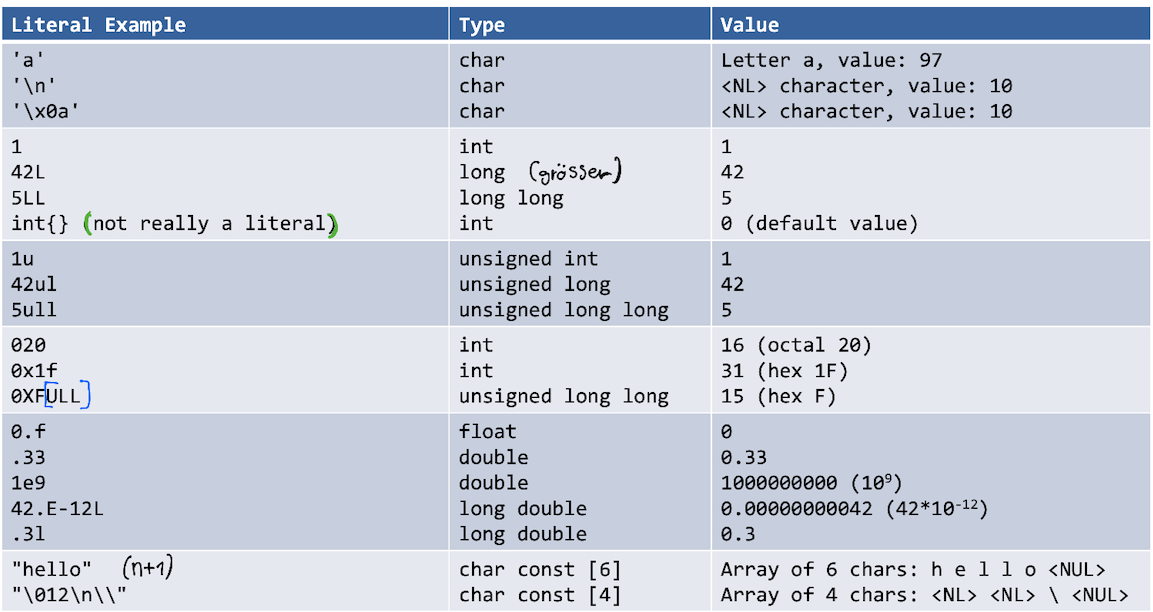
\includegraphics[width=0.75\linewidth]{images/literalexamples}
  \caption{C++ Variable Types}
\end{figure}

\begin{lstlisting}[language=C++]
(5 + 10 * 3 - 6 / 2) // precedence as in normal mathematics = 32
auto x = 3; / 3 // Fractions results of int operations always rundet down! 1
auto y = x%2 ? 1 : 0; // int boolean conversion 0=false, others are true.=1
\end{lstlisting}

\subsection{Const}
\begin{itemize}
  \itemsep -0.5em 
  \item Const should be used as often as possible, because it optimises the code.
  \item Const is comparable with the final from Java, although it has a higher guarantee that the variable is not changed.
  \item Const variables must be initiaized!
  \item To set const vars at compile time the keyword "constexpr" must be used.
\end{itemize}

\subsection{Auto}
The keyword auto can be used to deduct the type of a variable automatically at the declaration.
\begin{lstlisting}[language=C++]
auto const yearOfBirth = 2049; // int
auto const name = "Rick Deckard" // std::string
\end{lstlisting}

\subsection{Strings}
 std::string is C++'s type for representing sequences of char (which is often only 8 bit). This Strings are mutable in C++ in contrast to Java. Literals like "ab" are not of type std::string they consist of const chars in a null terminated array.
 
 To have a std::string we need to append an s. This requires using namespace std::literals;.
 
 \begin{lstlisting}[language=C++]
 void printName(std::string name) {
	using namespace std::literals;
	std::cout << "my name is: "s << name;
}	
\end{lstlisting}

\textbf{String Capabilites}\\
 You can iterate over the contents of a string.
\begin{lstlisting}[language=C++]
void toUpper(std::string & value) {
	for (char & c : value) {
		c = toupper(c); 
	}
}	
\end{lstlisting}
\pagebreak


\section{Streams}
\begin{itemize}
  \itemsep -0.5em 
  \item In the header files the inclusion of \lstinline[language=C++]{#include <iosfwd>} forward declaration header. This is sufficient for function declarations.
  \item In a source file for "std::cin" and "std::cout" the \lstinline[language=C++]{#include <iostream>} should be used. This containts all the definitions needed for "std::cin" etc. If just one of the two stream objects is need use either \lstinline[language=C++]{#include <ostream>} or \lstinline[language=C++]{#include <istream>}. The last two dont include the "std::cin" and "std::cout".
  \item In the main function "std::cin" and "std::cout" is used with the corresponding shift operators "<<", ">>".
  \item "std::istream" objects do return false if we are in an invalid stream state.
  \item "std::endl" flushes a buffered out stream. Better use "\textbackslash n". 
\end{itemize}

\subsection{Input and Output Streams} 
Functions taking a stream object must take it as a reference, because they provide a side-effect to the stream (i.e., output characters).

\textbf{Simple I/O} \\
Stream objects provide C++'s I/O mechanism with the help of the pre-defined globals: std::cin std::cout. Streams have a state that denotes if I/O was successful or not.
\begin{itemize}
  \itemsep -0.5em 
  \item Only .good() streams actually do I/O
  \item You need to .clear() the state in case of an error
  \item Reading a std::string can not go wrong, unless the stream is already \lstinline[language=C++]{!good()}.
\end{itemize}

\textbf{Reading a std::strting Value }
\begin{lstlisting}[language=C++]
#include <iostream> 
#include <string>
	std::string inputName(std::istream & in) {
		std::string name{};
		in >> name;
		return name; 
}	
\end{lstlisting}
\textbf{Reading an int Value}
\begin{lstlisting}[language=C++]
int inputAge(std::istream& in) {
	int age{-1};
	if (in >> age) { // Boolean conversion
	return age; 
	} 
	return -1;
}
\end{lstlisting}
\textbf{Chaining Input Operations}
\begin{itemize}
  \itemsep -0.5em 
  \item Multiple subsequent reads are possible 
  \item If a previous read already failed, subsequent reads fail as well
\end{itemize}

\begin{lstlisting}[language=C++]
std::string readSymbols(std::istream& in) {
	char symbol{};
	int count{-1};
	if (in >> symbol >> count) {
		return std::string(count, symbol); 
	} 
	return "error";
}
\end{lstlisting}

\subsection{Stream States}
Formatted input on stream  is must check for is.fail() and is.bad(). If failed, is.clear() the stream and consume invalid input characters before continue.

\begin{figure}[h!]
  \centering
  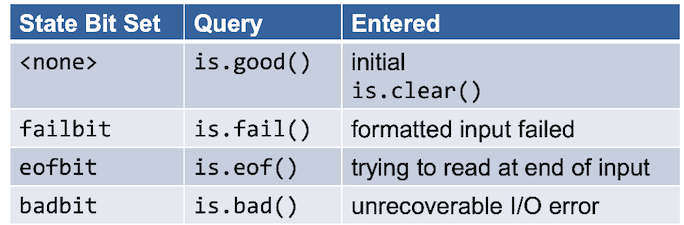
\includegraphics[width=0.7\linewidth]{images/streamstates}
  \caption{Stream States in C++}
\end{figure}

\subsection{Manipulators}
For the formatting of the output a vide variety of manipulator can be used.
% TODO add some manipulators


\pagebreak
